\documentclass{kththesis}

\usepackage{graphicx} % figures
\usepackage{csquotes} % Recommended by biblatex
\usepackage{biblatex}
\usepackage{mathtools}
\usepackage{listings}
\usepackage{xcolor}
\usepackage{caption}
\usepackage{subcaption}

\addbibresource{references-extra.bib}
\addbibresource{references.bib} % The file containing our references, in BibTeX format

\title{Robot-human handovers learning of novel objects through autonomous learning}
\alttitle{Inlärning av robot till människa överlämningar genom autonomous learning}
\author{Simon Simonsson}
\email{simonsim@kth.se}
\supervisor{Christian Smith}
\examiner{John Folkesson}
\programme{Master in Computer Science}
\school{School of Electrical Engineering and Computer Science}
\date{\today}

\begin{document}

\frontmatter % Frontmatter includes the titlepage, abstracts and table-of-contents
\titlepage

\begin{abstract}
	english abstract
\end{abstract}

\begin{otherlanguage}{swedish}
	\begin{abstract}
		svensk sammanfattning
	\end{abstract}
\end{otherlanguage}

\tableofcontents

\mainmatter % Mainmatter is where the actual contents of the thesis goes

\chapter{Introduction}
\section{Background}

There are many different scenarios where we could imagine we would draw advantage of a robot performing handovers to a human. In an industrial environment, to save human workers the time of fetching tools by themselves, a robot could be employed for the task of handing over the tools when needed. In another scenario a robot could be employed into helping a human with a physical disability into reaching different things around the home. Different objects require different grips and/or movements to perform the actual handover. We can not for example hand over a sharp knife the same way that we hand over a pen, nor a hammer the same way we would for a cup of hot coffee. A challenge with robot-human handovers is to get the robot to perform the handover correctly depending on the object in question. In an industrial environment the number of tools that the robot is to handover is finite, and it is possible to train it for each one of the tools. However in the home of someone with a disability there is almost an infinite amount of different objects that can require handovers and it would be very inefficient to train the robot for each one of them. Existing methods for determining proper handover movements relie on robot-computed configurations and preprogrammed object-specific information. These methods all require data over correct hand grip and movement connected to objects as mentioned in this article [section IV.C]. With this work we would like to propose a way for a robot to determine grasp and handover methods purely from observations, in the goal of making it able to adapt to new objects without any prior knowlegde about grasp configurations.

\section{Research questions}
\label{sec:research_questions}

In this work we want to see if we can develop a system for a robot to learn autonomously how to handover over a series of different objects without labeling the data, and if it can apply this to novel objects that it has not seen. We will be answering questions such as if there is a way to classify handovers and if there is a link between object properties and a type of handover. Later we will see if this is applicable to new objects.

With this project we will try to answer the following questions:
\begin{itemize}
	\item Are we able to classify objects by their handover settings?
	\item Can we relate the visual aspects of an object to its class?
	\item Is this model applicable to new objects?
\end{itemize}


\chapter{Related work}
\section{Handovers}
% handovers and research around it
Object handovers is a process that involves many parameters. Object grasping, timing of social cues and head gaze are just a few to mention some. Studies suggest that humans prefer a minimum jerk, human-like motion when being handed over an object \parencite{Huber2008} \parencite{Huber2008a}. As a consequence other research has set their focus on observing humans as to identify these parameters that affect a handover and their importance, with the aim of having robots immitate humans. \textcite{Moon2014} found that only by imitating human gaze cues during a handover the robot can help the human reach for the object sooner, even before the robot finishes the movement.

\textcite{Huang2015} researched adaptation between humans in collaborative tasks, concluding that adaptevily coordinating actions can increase performance in tasks such as handovers between robots and humans. The work of \textcite{Chan2015} found through a user study of handovers under different conditions that natural handovers may differ from receiver-oriented handovers, showing us that robots would need to take this into account when learning from demonstration to make sure it puts the human interests in priority.

Although \textcite{Koene2014} found through their research that a fast motion from the robot was better received from the human side than a spatially accurate end position of the robotic grasp, \textcite{Admoni2014} showed through their experiments that introducing some deliberate delays in the handover helps the receiver with focusing on the robot's head (i.e. gaze) and understand better its suggestions, which was also proposed by \parencite{Moon2014}.

\begin{figure}
	\centering
	\includegraphics[width=0.5\textwidth]{img/related-work/planning-simulation.png}
	\caption{Human detection phase and handover planning in simulated environment in \parencite{Aleotti2012}.}
\end{figure}

\section{Grasping}
% grasping
A very important feature as to ensure the success of a handover, is the grasping of objects. Robotic grasping is itself a widely researched topic and several models have been proposed to compute proper grasping of objects. Some examples of previous work that attempt at defining the representation of the object and its features for the task of grasping include \textcite{Miller2003} who decompose an object into primitive shapes to identify good grasping points (seen in figure \ref{fig:rel__shape-primitives}), while \textcite{Huebner2008} use a Minimum Volume Bounding Box solution to do the same (seen in figure \ref{fig:rel__mvbb}). \textcite{Morales} represent objects by nine different high level descriptors of data and developed a learning framework upon this.

Just as with handovers, in the domain of grasping several studies have been conducted as to observe human grasping as to make robots immitate them. \parencite{Cutkosky1990} \parencite{Feix2009} \parencite{Kang1993} made taxonomies for different grasp choices used by humans depending on objects and tasks. For the task of handovers, some research tried associating correct grasping of objects with their type and its affordances (\parencite{Song2015}, \parencite{Chan2014}) where by associating an object with different ways of manipulating it we identify a grip which is best suited when handing it over as to increase productivity for the receiver. Seeing how force closures are usually quite limited in terms of mobility (at least relative to the human hand), this thesis will not concentrate on the actual grasping and just leave it as future work after the correct grasping region has been identified as shown in figure \ref{fig:grasp-representation}. Please refer to the work in \parencite{Sahbani2012} for a complete review of the possibilities for robotic grasping.

\begin{figure}
	\centering
	\includegraphics[width=0.3\textwidth]{img/related-work/shape-primitives.png}
	\caption{From \parencite{Miller2003}: A mug model and its primitive representation.}
	\label{fig:rel__shape-primitives}
\end{figure}

\begin{figure}
	\centering
	\includegraphics[width=0.5\textwidth]{img/related-work/mvbb.png}
	\caption{From \parencite{Huebner2008}: Minimum Volume Bounding Box on Homer model.}
	\label{fig:rel__mvbb}
\end{figure}

\begin{figure}
	\centering
	\includegraphics[width=0.3\textwidth]{img/related-work/grasp-representation.png}
	\caption{A five-dimensional grasp representation with terms of location, size and orientation. The blue lines demark the size and orientation of the gripper plates. The red lines show the approximate distance between the plates before the grasp is executed.}
	\label{fig:grasp-representation}
\end{figure}


\section{Machine-learned systems}
\label{sec:machine_learned_systems}
% rule based algorithms vs machine learning
Within artificial intelligence applications there are several approaches that can be used. A common design for these systems has been by using \emph{rule-based algorithms}. In this case there are a set of rules, most often crafted by humans, dictating the behavior of the system depending on certain conditions. An other approach is to use \emph{machined learned} systems. This second way of designing the system is based on having the machine learn from a set of observations. The learning process can be different, but revolves mostly around fitting a statiscal model to the recorded observations as to be able to predict behavior in future observations.

\begin{figure}
	\centering
	\includegraphics[width=\textwidth]{img/related-work/ann.png}
	\caption{Feed-forward layered artificial neural network [79]. Input layer communicates to
one or more hidden layers where the actual processing is done, computing the weights (w). The
hidden layers then connect to the output layer. Each hidden layer have a certain number of
artificial neurons, which have a defined activation function that produces the output for the
next neuron \parencite{extremetech}.}
	\label{fig:rel_ann}
\end{figure}

There are many different models that can be applied for machine-learned systems, and a very common one of them are \emph{Artificial Neural Networks} (ANNs). These models take inspiration from the way the human brain processes information. ANNs consist of a number (a network) of interconnected neurons which compute and propagate their output through a series of layers. An example showing the basic idea can be seen in figure \ref{fig:rel_ann}. The term \emph{Deep Learning} refers to ANNs that have a large number of layers.

Machine-learned systems have for a long time been very limited in their ability to process raw natural data. Careful and intelligent preprocessing has been required as to transform this raw data into a smaller set of features that is easier for the machine to learn upon. This includes noise reduction, feature selection and dimensionality reduction, and makes the preprocessing step no easy task as it requires an expertise knowledge of the domain that the system is to be used within and can be very time consuming to make sure it becomes correct. This is also linked to the high requirements in processing power that comes with working with high-dimensional raw data. However, with the advancements in hardware, ANNs and deep learning systems through their large multi-layer setup are able to learn a hierarchy of features and are making large progress within machine-learned systems to perform representation learning from raw data, minimizing the amount of preprocessing \parencite{Lecun2015}. In the example of computer vision, deep neural networks would learn how to extract global features such as edges from the image, and through the layers work on more complex features within the patches extracted from the previous layer.

Convolutional Neural Networks (CNNs) are a class of ANNs within deep learning that have a special architecture designed to process raw data that comes in multiple arrays such as the color channels in images which make them popular within computer vision. CNNs are structured as a series of stages where the firsts ones are usually composed of layers of type convolutional and pooling, with the goal to detect local conjuctions of features from the previous layer (\parencite{Lecun2015}, \parencite{Jarrett2009}). With minimal preprocessing CNNs can learn a variety of high- and low-level features to perform with great accuracy several tasks within visual recognition. \textcite{Lee2009} demonstrate through unsupervised learning of a convolutional network how the network learns in the early layers edge detection and object parts. \textcite{Turaga2010} show by emphasizing the learning stage, the CNN is able to learn edge detection with mininum pre- or postprocessing.

The perfomance of all types of ANNs is linked to their architecture. Changing the number of layers or their sizes can result in large fluctuations in performance, for the better or the worse. Some architectures become overtime more well-known for their success at certain tasks. One of them, named AlexNet, is the one published by \textcite{Krizhevsky2012} which achieved great results at the \textcite{ImageNet} image classification challenge LSVRC-2010. In their work they credit the performance of their neural network to its deep structure of many layers, showing that by only removing one of the convolutional layers its performance would decrease with about 2\%. Figure \ref{fig:alexnet_orig} illustrates the network architecture of AlexNet.

\begin{figure}
	\centering
	\includegraphics[width=\textwidth]{img/methods/alexnet_original.png}
	\caption{AlexNet architecture.}
	\label{fig:alexnet_orig}
\end{figure}

Machine-learned applications are becoming more and more frequently used because of their high performance, lower requirements for human intervention, as well with how it has become increasingly easy to collect and represent data in a more versatile way. The works in \parencite{Aleotti2012} \parencite{Suay2015} \parencite{Kim2004} all report good results for handovers between robots and humans, but are supported by rule-based algorithms. Rule-based algorithms can present some limits of adaptation to a wider spectrum of scenarios than those thought of when the algorithm was created. They can as well become error prone because of human factors. \parencite{Redmon2014} \parencite{Lenz2015} \parencite{Jiang2011} \parencite{Huebner2008a} are examples of work that instead use the advantages of machine-learned models to achieve good results, avoiding dictating the rules for grasping and handovers themselves. One disadvantage does nonetheless persist with these methods, which is the fact that their datasets for training require the time consuming task of manually labeling.


\section{Autonomous learning}


\subsection{Supervised and unsupervised learning}

Classification consists of creating a statistical model to determine the group (i.e. class) an observation belongs to. For machine-learned systems this requires them to find the connection between the features connected to an observation and their respective group. To achieve this we can use two different aproaches: \emph{supervised} or \emph{unsupervised} learning.

Supervised learning uses a dataset that is labelled, meaning that the observations within it are correctly assigned from the beginning. In this case we fit our model to the observations and their known label. On the contrary, in unsupervised learning any grouping of the observations is uknown to us. In this method we use cluster analysis to compute relationships between observations based on different metrics, and group them accordingly.

\emph{Autonomous learning}, also known as \emph{semi-supervised learning}, is a method of combining the two prior methods. Through unsupervised learning, groups are created for the observations and with a supervised learning algorithm a model is created to predict the group for future observations.


% learning from demonstration
\subsection{Learning by demonstration}

\begin{figure}
	\centering
	\includegraphics[width=\textwidth]{img/related-work/demonstrations.png}
	\caption{From \parencite{Chan2015a}: Stages of extracting grasp configurations from handover demonstrations. A - Object detection. B - Human detection and tracking. C - Grasp point detection. D - Direction of torso-to-hand vector for handover cue detection. E - Object orientation at handover.}
	\label{fig:rel__demonstration}
\end{figure}

\begin{figure}
	\centering
	\includegraphics[width=\textwidth]{img/related-work/cnn-architecture.png}
	\caption{Full architecture used by \textcite{Redmon2014}.}
	\label{fig:rel__cnn-arch}
\end{figure}

A less explored research field is yet to teach robots grasping and handovers by demonstrations using vision. Having robots learn by observing humans would enable faster collection of data, save time from manually labeling and allow the robot to use more human-like motions. Common within robot simulation is that the data required for processing is represented by 3D models of the objects and environment (for example in \parencite{Miller2003}) which are not trivial to come by for newly encountered objects in a live setting as it would require the robot to see everything from all angles. Another factor is the accuracy of sensors and quality control of the data (i.e was it as good handover?) are some of the limitations of learning from observations which makes it a challenging method. Kinect sensors have become popular within robotics today because of their relatively low cost and support for depth data which can help in creating three dimensional renderings of images. \parencite{Lenz2015} \parencite{Redmon2014} \parencite{Jiang2011} \parencite{Saxena2008} are example of works that propose methods for training and identifying grasp sites using RGBD images recorded by a stereo camera, but the problem with these works is that they do not train on data collected by demonstrations without manual annotation. \textcite{Chan2014} collected data by observing humans interacting with objects, but the data covered other scenarios of object interaction than handovers. \textcite{Strabala2013} trained a model using decision trees from recorded data of humans performing handovers, but they had to manually label the recorded material with eye-gaze, two-dimensional position of participants, object locations and handover positions. \textcite{Chan2015a} do however propose a framework for robots to learn handovers and grasp sites through demonstration as seen in figure \ref{fig:rel__demonstration}. By handing objects to a robot they then have the robot repeat the handover in reverse order back to the human. They however do not have the robot learn any object features as to associate the handover settings to it, for the purpose of predicting the handover settings for new objects.


% new objects
\subsection{Foreign objects}

One of the challenges within robotic grasping and handovers is the ability to perform their task on an object that the robot has never seen nor been trained for. Some previous research do enable grasping of foreign objects, but requires a lot of data which itself needs to be labeled. For example \textcite{Huebner2008a} in a continuation of their work in \parencite{Huebner2008}, train a neural network that can be used for grasping of novel objects, but requires the network to be trained on a previously manually labeled dataset of grasps. Also the proposed model by \parencite{Chan2014} requires data on different ways to manipulate an object before the robot can calculate a way of grasping it and handing it over, making it hard to deploy in a new environment. Complete and accurate 3D models are unfortunately not always available and not feasible in an environment where a robot should learn from observing humans.

% how to use this related work for this thesis
\textcite{Redmon2014} show very promising results with their implementation in finding grasp sites on objects, even for those that are not present in the training set, illustrating the high performance of convolutional neural networks. Their work is based on the ImageNet model that was further trained with RGBD images for detecting grasp regions. The ImageNet model is however trained for RGB images, the authors solved this by dropping the blue channel and replacing it with the depth data. In figure \ref{fig:rel__cnn-arch} we can find an overview of the full architecture for their network. The problem is that the data that it needs for training is manually annotated. The framework proposed in \parencite{Chan2015a} is a good starting point for the collection of data as to train a model that can be later used for grasping and handovers. This thesis will try and combine these works by implementing a framework for collecting data through demonstration from humans and process it as to train a convolutional neural network that can later identify grasping sites and handover features on foreign objects through RGBD images.


\chapter{Methodology}
\section{Overview}

The goal of this project is to develop a system that autonomously learns handover settings for objects by observation. Given an image of an object, we want the system in the end to be able to output its settings for a handover. Another of our requirements is that the learning has been abstracted enough that this system is accurately applicable on new objects that are not present in the training set.

One way to go about with this would be by learning the handover settings for an object and then fitting a model to recognize the object (i.e. object classification). In other words, record all the handover features for each individual object, create a mean from them, and train a model to recognize the object based on images as to output its settings. Such a model would for \(n\) number of objects need to learn to output \(n\) different classes. This can potentially become an increasingly difficult task as the number of objects grows, because with that the requirements on the size of the data set grows. Such a system would believe that each object has its own unique settings, and might not be scalable to other objects absent from the training set.

If we instead hypothesize that some objects are handed over in similar fashion depending on their visual features we can try a different approach: letting the system by itself find relationships between the observations of handovers and through this classify the individual objects into classes of handovers. After that the system is tasked with finding visual similarities between the objects that define which class they have been assigned. In theory this simplifies our problem as the number of outputs should shrink. We no longer pressure the system into properly recognizing individual objects but instead similarities, which also lowers the requirements on data collection.

\begin{figure}
	\centering
	\includegraphics[width=\textwidth]{img/methods/flowchart.jpg}
	\caption{Flowchart describing the work process. Red delimiter marks where the first part of the works goes over to the second part.}
	\label{fig:flowchart}
\end{figure}

In figure \ref{fig:flowchart} the workflow is summarized. The first part of this work will be to observe and record a number of handovers between humans for a defined set of objects which the system will try to categorize into different classes. In a second part each object will then be assigned a class that we train a model to return when given an image of the same object. Seeing how we do not have any labels for the handovers, but still want to train a model that outputs some defined class for how the object should be handed over, we will be using a semi-supervised approach in this project: by first applying an unsupervised learning algorithm to categorize and create classes of handovers that are later used as output for self-supervised learning.


\subsection*{Methods for answering the research questions}

\subsubsection*{Are we able to classify objects by their handover settings?}

This will be answered in the first part of our work where we try through an unsupervised clustering algorithm to classify the handover features of the objects. If for all objects, a majority of their samples belong to a specific cluster, then we deem it possible to do so.


\subsubsection*{Can we relate the visual aspects of an object to its class?}

The second part of the work is dedicated to analyzing image data of the objects. In case we can answer yes to the previous question we will find ourselves with groups consisting of several objects and want to know if the objects within a group are visually similar enough. By exploring if RGBD images alone are enough to successfully predict the handover class for the objects that are part of it, we will see if our model finds enough visual features in common between the objects to relate them to their class. If our model is accurate enough we can say that there are visual similarities between the objects belonging to the same class.


\subsubsection*{Is this model applicable to new objects?}

We want to know if our method is applicable for a larger set of objects where we only record and train for a small subset. In case we can answer yes to the previous question and we can make correct predictions for the training set, we are going to try on a test set consisting of foreign objects. These new objects will be manually classified depending on the results from the first part, and tested on the model achieved from the second part. With a high enough success rate we will consider our method as successful for new objects as well.


% Tools and material

\section{Tools and material}

\subsection*{Hardware}

During the project the following material were used:

\begin{description}
	\item[Kinect for Windows v2] Motion sensing device developed by Microsoft used for recording and taking pictures with support for color, depth and infrared data.

	\item[GeForce GTX 980 Ti] Nvidia brand GPU for better performance during training of for example deep neural networks that require a lot of data and processing power.

	\item[\textcite{AprilTags}] In order to extract data from the recorded frames about the objects we need to detect the objects themselves. Object detection is a very difficult part of computer vision and there are many different methods, where some are more robust than others to do so. To help with this part to make data extraction easier and more precise we will be taking help of AprilTags. AprilTags can be compared to QR-codes that are printed out on small papers and fastened onto the objects. With the help of their software library we can easily track the objects in the recorded material by getting the position of the four corners of the tag and its center, which enables us to estimate such things as pose of the object.

	\item[Fifteen different objects to be handed over] Chosen randomly around the house, all of which can be handed over using only one hand with ease. The set objects include: a knife, a screwdriver, a can, a box, a pair of cutters, a tube, a pitcher, a glass, a bottle, a brush, a cup, a hammer, a pen, a scalpel and a pair of scissors.

\end{description}

\begin{figure}
	\centering
	\includegraphics[width=\textwidth]{img/methods/apriltagrobots_overlay.jpg}
	\caption{Example of AprilTags in use on robots.}
\end{figure}

\subsection*{Software}

The applications were written in C++ and Python depending on availability of libraries. To implement the system the following software tools and programming libraries were used:

\begin{description}
	\item[\textcite{GIMP}] Image editing program that will be used for manual preprocessing of some images.

	\item[\textcite{libfreenect2}] Open source library written in C++ for communicating with the Kinect v2 camera.

	\item[\textcite{OpenCV}] Open source library for computer vision with bindings for C++ and Python, as well as other languages.

	\item[AprilTags programming library] C++ library written by the creators of AprilTag to help extract data from captured images such as the four corners of the tag and center of the tag.

	\item[\textcite{scikitlearn}] Python machine-learning library. Contains several useful tools for implementing and fitting models, as well as data processing.

	\item[\textcite{Tensorflow}] Open source Python library for creating and training neural networks with GPU support for more efficient processing time.

\end{description}


\section{Categorization of handovers}

\subsection{Recording of handovers}

For this purpose a number of volunteers were asked to be recorded while handing over a set of objects between each other. Even though Kinect v2 supports depth images, only two-dimensional color data will be used in this part. A total of eleven people who already knew each other from before volunteered (including myself) for this task. Pairs of volunteers were permuted as to try and make each person adapt to different receivers while being the giver. Instructions for handing over the objects were given prior to recordings as to make sure participants gave the object in a manner that the person receiving the object can use it straight away after grasping it. For example the hammer should be handed over with its handle first in a manner that the next person can start hammering directly without requiring a switch of grip after receiving it. Or a cup is to be handed handle-first so the person can start drinking right away. A bottle is easier to pour from if you hold it below its center of gravity therefore this area should be free for the receiving person while handing it over. For reasons that we will see later participants were instructed to use a grasp that covers the object, they could not for example hand something over flat in their palm. This is because of how the grasp region is identified and its limitations. The general regions of where to grasp by the giver and what part to present to the person receiving were chosen by myself with in mind for optimization for the receiver when given the object. For objects that might contain liquids the participants were asked to imagine that these objects were filled to the top while handing them over between each other.

\subsection{Extracting features}

% TODO write more about image moments
% TODO write about homography

\subsubsection{Orientation of the object}

The first set of features that we will extracted from the recorded material will be around the orientation of the object when being handed over, i.e. the transformation from its ground truth to the observed position. Before any work is done with the recorded material, for each object we manually create a reference image representing its ground truth position. The orientation of the ground truth was chosen to be the object's placement while in resting position (e.g for a bottle, standing up). For those objects that are laid down, their orientation was chosen to be with their head upwards. From these images we also generate binary masks that will be used to mask out the object after detection within the frames. Figure \ref{fig:objects_montage} shows the reference images created and figure \ref{fig:masks_montage} shows their binary masks. These images were created using the image manipulation software GIMP.

\begin{figure}
	\centering
	\includegraphics[width=\textwidth]{img/methods/objects.jpg}
	\caption{Ground truth images of the objects used with an AprilTag fastened to them.}
	\label{fig:objects_montage}
\end{figure}

\begin{figure}
	\centering
	\includegraphics[width=\textwidth]{img/methods/masks.jpg}
	\caption{Binary mask of each object.}
	\label{fig:masks_montage}
\end{figure}

One of our biggest challenges with the project is to actually detect the object in each frame. This is a very non-trivial task and there is much research around methods for object detection. To help us with this part of the project and ensure that the data we extract is accurate, we will use AprilTags. They can easily identify the four corners of the tags in a frame and by this way locate the object. Using the OpenCV library and their \texttt{findHomography} function, we can compute the homography matrix that transforms the four corners of the tag in the reference image to the corners of the tag found in the frame.

A homography matrix \(H\) is a 3x3 matrix with a total of nine values which creates quite a few features if we would try and cluster on it. Also it contains data on how to translate the object in three-dimensional space, which in our case is irrelevant as we are only working with two-dimensional data. Alternatively we can calculate a rotation of the object and through an angle represent its orientation with instead only one feature. As we are only working with two-dimensional data we will only interest ourselves for the rotation on the z-axis. Using the homography we can calculate a rotation matrix from which we can later derive the searched angle. Using the Python code presented in listing \ref{lst:rotation_matrix} based on the OpenCV library, we compute a 3x3 rotation matrix \(R\). Using this matrix we can compute the angle \(\theta_R\) as \(\theta_R = \arctan(R_{1,0} / R_{0,0})\). In this case the rotation will be around the center of the tag because it is from which we calculated the homography matrix.

\begin{lstlisting}[
	language=Python,
	frame=single,
	label={lst:rotation_matrix},
	caption={Python code to calculate rotation matrix from homography matrix using OpenCV and numpy libraries (taken from \parencite{OpenCVHomographyDemo}).},
	float,
	floatplacement=H,
	]
norm = np.sqrt(np.sum(H[:,0] ** 2))
H /= norm
c1 = H[:, 0]
c2 = H[:, 1]
c3 = np.cross(c1, c2)

R = np.zeros((3, 3), dtype=np.float64)
for i in range(3):
	R[i, :] = [c1[i], c2[i], c3[i]]
w, u, t = cv2.SVDecomp(R)
return np.dot(u, t)
\end{lstlisting}


\subsubsection{Grasp features}

The previously calculated homography matrix can be used to transform the object's binary mask, and then be applied on the frame as to mask out only the object. From this we can afterwards retrieve a grasp region of the object.

Skin color is a quick way of segmenting and finding grasp region as the color of skin is quite different from the colors of the objects, but the method is not too robust in covering many different people as the color can vary quite a lot from person to person. The setting for skin color had to therefore be tweaked manually depending on the participant. By using the homography matrix and the binary image, we have been able to mask out the object from the scene. This image of the found object is later segmented by skin color. A contour expressed as a rotated rectangle which represents our grasping region is then calculated around the largest segmented region found.

A rotated rectangle is composed of three different parameters: width, height and angle. Another possible feature we can extract is the ratio between area of grasp region and area of object. Using the binary image of the object we can compute its area \(A_{object}\) with the help of OpenCV by using \texttt{findContours} and \texttt{contourArea}. The area of the rotated angle is simply \(A_{grasp} = width \times height\) and the ratio between them becomes \(A_{ratio} = \frac{A_{grasp}}{A_{object}} \).

The last features that we can extract are: the distance \(\Delta\) as the L2 norm between centers of the grasp region \(O_{grasp}\) and center of mass of the object \(O_{object}\), and the direction between these centers. The center of mass can be computed using the image moments of the binary image. Moments are retrieved with the help of the \texttt{moments} function part of the OpenCV library, then the following formula gives us the center:

\[
	O_{object} = \frac{M_y}{M}, \frac{M_x}{M}
\]

We can then extract the distance between center of mass of the object and the center of the grasping region as a feature. We can also express this as a ratio to the length of the diagonal of the object. It also enables us to create a unit vector from the center of mass of the object towards the grasping region.

% TODO write better later
To summarize we can extract the following features:
\begin{itemize}
	\item Rotation of object in z-axis, extracted from the homography matrix of the AprilTag.
	\item Distance between center of mass of the object and the center of the grasping region.
	\item Ratio of distance between center of mass of the object and the center of grasp, over the diagonal of the object.
	\item Direction in x-axis between center of mass of the object and the center of the grasp.
	\item Direction in y-axis between center of mass of the object and the center of the grasp.
	\item Ratio of area of the grasping region by the area of object.
	\item Width of grasp region.
	\item Height of grasp region.
	\item Angle of grasp region.
	\item Center of grasp region.
	\item Center of mass of the object.
\end{itemize}

With these features we define for a robot how to grasp an object and present it to a human for a handover. This list of features is however quite large and represents a very high-dimensional set of data. High-dimensionality can become quite problematic as the values might not vary with the same amount in all dimensions as well as create similarities that are not there between objects. A first filtering of these features can be made on the idea that the features should be expressible invariant to the object, i.e. we only keep the features that are expressed in relation to the object. This will leave us with the following list:

\begin{itemize}
	\item Rotation of the object in z-axis, expressed between 0.0-1.0 where 1.0 is a full circle (360 degrees).
	\item Direction in x-axis between center of object and center of grasp.
	\item Direction in y-axis between center of object and center of grasp.
	\item Ratio of distance between center of the object and the center of the grasping region to the diagonal.
	\item Ratio area of grasp region over area of object.
\end{itemize}


\subsubsection{Filtering of unwanted frames}

One recording session consists of one pair of volunteers during which the one giving has handed over all objects in the set to the receiver. In this project we only interest ourselves for the features that define how an object is to be presented to the one receiving it, i.e. the actual moment in the end of the handover motion when the giver holds out the object ready for the receiver to take it. At all times of this session the application is continuously recording, creating a large number of frames that are of no interest such as when the participant handing over the objects is fetching the next one or the person receiving is putting one of them away. Some preprocessing of the frames is therefore required to find the frames of interest.

A first step is to create a Region of Interest (ROI) in which we will concentrate on searching for objects. This will not only help filter out the vast amount of frames that are not of interest, it will also help with performance as opposed to if we were searching the entire frame. Our ROI is arbitrarily set to the middle of the frame where the person handing over the object would finish the movement, and set to be large enough to detect the tag and see the entire object. When a tag is detected within the ROI we flag this frame to be a handover moment before extracting the features. This is unfortunately not enough because we might be flagging frames where the receiver is holding the object after taking it, or maybe both are holding it but the system detects the receiver's hand as the largest grasping region. Figures \ref{fig:handover_bottle} and \ref{fig:handover_hammer} demonstrate frames that the system detected as handovers with the objects masked out and the grasping region identified. The methods explained above might also give incorrect data if the grasping region was incorrectly detected. Manual filtering was later applied to images that were flagged as handover moments as to make sure they and the data extracted was correct. Figure \ref{fig:handover_incorr} illustrates a situation that needs to be manually filtered out when the system perceives to have identified a handover situation but the grasping region identified is that of the receiver's.

\begin{figure}
	\centering
	\begin{subfigure}[t]{\textwidth}
		\centering
		\includegraphics[width=\textwidth]{img/methods/handovers/bottle_frame.jpg}
		\caption{Handover of bottle.}
		\label{fig:demo_handover_bottle}
	\end{subfigure}
	\par\bigskip
	\begin{subfigure}[t]{0.5\textwidth}
		\centering
		\includegraphics[width=\textwidth]{img/methods/handovers/bottle_masked.jpg}
		\caption{Bottle masked out and grasp region identified.}
		\label{fig:handover_bottle_masked}
	\end{subfigure}
	\caption{Handover demonstration of a bottle with the grasp region detected after being masked out. The giver was instructed to pretend like the bottle was full of liquids to make sure they held it upright.}
	\label{fig:handover_bottle}
\end{figure}

\begin{figure}
	\centering
	\begin{subfigure}[b]{\textwidth}
		\centering
		\includegraphics[width=\textwidth]{img/methods/handovers/hammer_frame.jpg}
		\caption{Handover of hammer}
		\label{fig:demo_handover_hammer}
	\end{subfigure}
	\par\bigskip
	\begin{subfigure}[b]{0.5\textwidth}
		\centering
		\includegraphics[width=\textwidth]{img/methods/handovers/hammer_masked.jpg}
		\caption{Hammer masked out and grasp region identified.}
		\label{fig:handover_hammer_masked}
	\end{subfigure}
	\caption{Handover demonstration of a hammer with the grasp region detected after being masked out. The giver was instructed to give it handle first, holding the head so the receiver is able to use it straight away.}
	\label{fig:handover_hammer}
\end{figure}

\begin{figure}
	\centering
	\begin{subfigure}[b]{\textwidth}
		\centering
		\includegraphics[width=\textwidth]{img/methods/handovers/incorr_frame.jpg}
		\caption{Handover of the hammer after the receiver takes the object.}
		\label{fig:demo_handover_incorr}
	\end{subfigure}
	\par\bigskip
	\begin{subfigure}[b]{0.5\textwidth}
		\centering
		\includegraphics[width=\textwidth]{img/methods/handovers/incorr_mask.jpg}
		\caption{Hammer with the grasp region of the receiver identified.}
		\label{fig:handover_incorr_masked}
	\end{subfigure}
	\caption{Example of frame with false positive. The object is detected within the region of interest but the identified grasping region is not that of the giver, but the receiver's.}
	\label{fig:handover_incorr}
\end{figure}


\subsection{Clustering by handover features}

After observing a number of handovers between humans, a first step is to try and categorize these handovers into different classes that can be applied for the objects. As we do not have any labels, or even unsure how many different categories of handovers we have recorded, we will attempt at clustering using an unsupervised learning algorithm by the features that we have extracted from the recorded material.

\subsubsection{K-Means} % TODO references

For the purpose of categorizing the handover samples we will be using the \emph{k-means} algorithm. K-means is an algorithm that attempts to classify a number of observations into \emph{k} number of clusters. The algorithm starts by creating \emph{k} number of centroids for each cluster and assigning our samples to the centroid within shortest distance. The algorithm iteratively then updates the centroids to become the mean of the samples assigned to it, and then re-assigns all samples depending on the new centroids. This is repeated either a fixed number of times or until the algorithm converges minimizing the sum of squared distances within the clusters.

We are faced with the problem that we do not know in advance how many clusters are best suited in this case. We will run k-means for a range of different number of clusters between two and fifteen, thereafter we will use the \emph{elbow method} and the mean \emph{silhouette coefficient} to decide what is the best fit.

The more clusters you have the better it would fit your data. Imagine that you had the same number of centroids as samples, you will in this case have a perfect fit because all samples would have a distance of zero to the centroid. On the other hand what we really are searching for is the \emph{fewest} number of clusters that gives the best "reasonable" fit. While starting with a small number of clusters and then gradually increasing the number step by step, we can observe how the sum of distances between the samples and their assigned centroid gradually decreases. When the gradient from one observation to the next is below a certain threshold, we deem the observation as a good a fit. An observation being here the results from clustering with a certain number of centroids. This is referred to as the \emph{elbow method}.

The formula for the \texttt{silhouette coefficient} of a sample is as following:

\[
	\frac{(b - a)}{max(a, b)}
\]
\[
	a = \text{distance from sample to assigned centroid},
\]
\[
	b = \text{distance from sample to nearest centroid other than assigned one}
\]

Silhouette coefficients range from -1 to 1. 1 is the best score because ideally the distance to the centroid is close to zero (\(a = 0\)) which would give us \(b / b = 1\). A score of zero indicates that some clusters might overlap each other, and a negative value shows a sample that has been assigned the wrong cluster. By looking at the mean silhouette coefficient of all samples, we can choose the number of clusters that maximizes the mean value.

Neither the elbow method nor the mean silhouette coefficient are enough by themselves to make an accurate decision on the number of clusters, but together they give us a very good estimate. We will therefore start by looking at the mean squared distances of the samples to their centroids and using the elbow method to define a possible interval of good fits for number of clusters, and after use the mean silhouette coefficient for the interval to make a decision.


\subsubsection{Principle component analysis (PCA)}

A challenge that presents itself using clustering algorithms is choosing what features are to be used for the purpose. All features are not equally important into classifying the samples. \textcite{Ding2004} showed in their work through principal components and K-means, the relevance between unsupervised dimension reduction and unsupervised learning. We will be using \emph{Principle component analysis} (PCA) to evaluate which features that are to be used to define each cluster. Ideally we use the smallest number of features possible, but also the ones that create the most distinct clusters. PCA defines the principal features as those with the highest variance. It reduces the dimensionality by calculating the variance over all dimensions, i.e. features, and either chooses a fixed number of the highest ones or keeps those that represent a certain ratio of the total variance within the data.

For this work we will be using PCA and try to reduce the dimensions of the handover data from five to three aiming on keeping a minimum of 80\% of the variance. In the case we have 80\% of the variance over three dimensions, the two that are left would not represent more than 10\% each, which is of low significance compared to the others.

%
% Prediction of handover class
%


\section{Prediction of handover class}

As mentioned our aim in the end is to have a robot be able to predict a handover setting given an image of an object. In our case we will have it predict a class of handovers which are the result of the previous clustering. The system needs in this case to be able to relate visual features that come through imagery to the class, also in a sufficiently abstract way that it can accurately predict the class for an unencountered object during training.

\subsection{Convolutional Neural Networks}

We hypothesize in this case that there is a number of features that can be retrieved visually from the objects, that define which class of handovers it belongs to. Even though we could try and preprocess all sets of objects and re-define them as a set of features, such as decomposing them into geometrical shapes, choosing which features it should be and how to retrieve them would be a challenging task, especially before knowing the results of the clustering. In section \ref{sec:machine_learned_systems} we mentioned convolutional neural networks and works such as \parencite{Lee2009}, \parencite{Turaga2010} where the layers through training are able to hierarchically extract features in the images to later perform precise visual tasks. This ability of CNNs corresponds well with our goal to have the machine learn autonomously without human preprocessing or labeling. Through fitting on a data set of images, our hope is that the machine will be able to draw relations between visual features extracted from the images with a certain class of handovers.

\subsection{AlexNet network}

For the task of predicting handover class from an image we will be training a convolutional neural network. The most challenging part with all artificial neural networks is to define their architecture. Changes to the number of layers and their sizes can play a significant role on the outcome of the results. Within object classification there have been a number of architectures proposed that have achieved good results, one of these is the \emph{AlexNet} network which was mentioned in section \ref{sec:machine_learned_systems}, and we will use as basis for our own network.

The AlexNet was designed for the ImageNet object classification problem in 2010, trained over 1,2 million images to output 1000 different classes. As a reminder, figure \ref{fig:alexnet_orig} shows the network architecture used by the AlexNet. It includes in total eight layers, all of which use ReLU non-linearity as activation function:

\begin{description}

	\item[Five convolutional layers] The first convolutional layer filters the \(224 \times 224 \times 3\) input image with 96 kernels of size \(11 \times 11 \times 3\) with a stride of 4 pixels. The second convolutional layer takes as input the (response-normalized and pooled) output of the first convolutional layer and filters it with 256 kernels of size \(5 \times 5 \times 48\). The third, fourth, and fifth convolutional layers are connected to one another without any intervening pooling or normalization layers. The third convolutional layer has 384 kernels of size \(3 \times 3 \times 256\) connected to the (normalized, pooled) outputs of the second convolutional layer. The fourth convolutional layer has 384 kernels of size \(3 \times 3 \times 192\) , and the fifth convolutional layer has 256 kernels of size \(3 \times 3 \times 192\).

	\item[Three fully connected layers] with 4096 neurons each, where the last one is fed to a 1000-way softmax output.

\end{description}

In total the network consists of 60 million parameters and 650 000 neurons. At the time, the designers of the network were under the restriction of the performance of GPUs, hence the parallel system. Seeing how our classification problem is of significantly smaller scale its size will do without problem, note however that we will re-design it so it runs sequentially on one GPU. The only other modification we will attempt will be by adding a new fully connected layer at the end with size depending on the results from the prior clustering. Figure \ref{fig:method_cnn_arch} shows our network architecture. As a side note: since the AlexNet network was designed, several other successful network architectures have been proposed, some that even outperform AlexNet. Such as \emph{VGG-16} by \textcite{Arge2015} and \emph{Inception} by \textcite{Szegedy2014}. These networks are however larger and deeper which would in theory require more processing time and as well as more data to fit, both which are of limited supply in this project. The AlexNet therefore makes a good compromise and should still be well suited for our smaller problem.

\begin{figure}
	\centering
	\includegraphics[width=\textwidth]{img/methods/network.png}
	\caption{Final version of the architecture. Serial version of the AlexNet architecture with an extra fully connected layer that has the same N number of outputs as the results from the clustering.}
	\label{fig:method_cnn_arch}
\end{figure}

\subsection{Training and testing}

We want the machine to learn from the handovers between humans that it has observed. We will therefore only use as our data set the objects that were used for recording handovers. Despite their potential for performing very well, one issue with ANNs (especially very deep ones) is that they often require a lot of data to do so. The amount of data we are able to gather by taking images of the objects is unfortunately not enough for a network as large as the AlexNet network which was designed for over a million images. Fortunately for us there are pre-trained weights to be found that we can work upon and increase our chances of success. At \parencite{AlexNetImplWeights} we can find a set of pre-trained weights to use and also we can find a good base for our own implementation of the architecture using the Python library \texttt{tensorflow}.  Next step is to fine-tune the pre-trained weights to better fit our own data and fit it to our desired output.

Color images contain three channels of color (RGB) to define their texture. We theorize that it is not only the texture that defines the visual features of a handover class but also the shape of the object. Three channels of color can therefore feel redundant if the color is not the only thing that defines what the objects have in common. It can also create distinctions between the objects that are unnecessary and maybe confusing for the network to learn as it will make it harder to learn relations between them. Depth data gives a good 2,5-dimensional representation of the shape of the object, which can also be visualized by converting it to a gray-scale image. This can be seen as one channel of color. As input data we will be taking inspiration from \parencite{Redmon2014} and perform the same alterations to our own data set by replacing the blue color channel with the depth image. Figure \ref{fig:rgbd} shows an example of the hammer with its RGB image to the left, depth image in the middle and to the right the color image with the blue channel replaced for the depth data. Using the Kinect v2 camera, both color and depth images were taken of all objects from several different angles in different positions. Data augmentation was later performed on the resulting images to enlarge the data set by using flipping, random cropping and random rotations of the images.

There are issues like black triangles in the corners or along the edges after rotating and/or cropping. These images are unwanted as the network might identify these regions with the objects. Therefore all the images created through data augmentation will be gone through manually as to make sure they are all suitable for training by the network. After we are done selecting images for our data set we are not guaranteed that it is balanced between the objects or the classes. To prevent any overfitting we will also make sure that we balance the data set evenly over all objects and classes.

\begin{figure}
	\centering
	\begin{subfigure}[b]{0.3\textwidth}
		\includegraphics[width=\textwidth]{img/methods/rgbd/rgb.jpg}
	\end{subfigure}
	\begin{subfigure}[b]{0.3\textwidth}
		\includegraphics[width=\textwidth]{img/methods/rgbd/depth.jpg}
	\end{subfigure}
	\begin{subfigure}[b]{0.3\textwidth}
		\includegraphics[width=\textwidth]{img/methods/rgbd/rgbd.jpg}
	\end{subfigure}
	\caption{RGB-, depth- and RGB-image with blue channel replaced by the depth data for the hammer.}
	\label{fig:rgbd}
\end{figure}


\section{Testing}
\label{sec:testing}

The training and validation of the model will be done on images from the objects that were used for training. This is to validate how well the model performs on objects that it has been trained for.

For testing purposes a number of images will be taken of objects that are not part of the training set. This is to see how well the model abstracts to other objects than the ones that it was trained on. On the contrary to the objects used for training we will not record handovers for these. Instead we will manually decide which class they belong to. This means that we are required to choose objects that in some ways resemble the objects from the training set and that have a quite decisive way of being handed over, so it does not become too questionable about which class they belong to. These objects are chosen depending on the results achieved from the clustering, further explanations are presented in section \ref{sec:res_setup}. The list of objects used for testing is as follows:

\begin{itemize}
	\item Beer glass.
	\item Bottle, a larger one than the one trained on.
	\item Carafe.
	\item Cup, different from the one trained on.
	\item Fork.
	\item Glass, with different shape from the training set.
	\item Knife, smaller and different shape than the one trained on.
	\item Scissors, smaller than the one trained on.
	\item Spatula.
	\item Spoon.
	\item Wine glass.
	\item Wooden spoon.
\end{itemize}

The images of the objects will be fed to the model and the accuracy will be tested against it. As there are no other methods to measure against we set as an aim of this project to reach an accuracy of 90\% with a standard deviation of 5\%. If these results are achieved we judge the model to be successful.


\chapter{Results and discussion}
% ======================================================================================
% CLUSTERING
%
% graphs to insert:
%	- score vs silhouette coefficient per cluster
%	- sample silhouette values for the best number of clusters
%	- 3D/2D cluster representation for the best number of clusters
% tables to insert:
%	- PCA outcome of the features
%	- object to cluster assignment depending on number of clusters (the best ones)
%	- cluster sizes depending on number of clusters
% figures:
%	- mean values of the features per cluster applied to the object


\section{Clustering}
Here we report the results from clustering depending on different features used.

%\begin{figure}
	%\centering
	%\includegraphics[width=\textwidth]{img/results/object_handovers.jpg}
	%\caption{Resulting handover data applied to each object}
	%\label{fig:object_handovers}
%\end{figure}


\subsection{Principal Component Analysis}


\subsection{K-means}

\input{tex/plot_scores.tex}

\input{tex/plot_silhouette_5.tex}

\input{tex/plot_silhouette_6.tex}

\input{tex/plot_silhouette_7.tex}

\input{tex/plot_clusters.tex}

\subsection{Object cluster assignments}



% ======================================================================================
% CLASSIFICATION
%
% GRAPHS:
%	- loss per step
%	- accuracy per step (validation and testing)
%	- training speed
% TABLES:
%	- confusion matrix
%	- accuracy per object
%	-

\section{Classification}
Output different results from classification depending on which layers are trained further and network architecture.



\chapter{Conclusions and future work}
\section{Conclusions}

In this work we introduced a model for a system to learn proper handover settings for objects through observations of handovers performed by humans. We showed that we can classify objects depending on a set of features extracted at the moment of the handover. By training a network to output a handover class based on an image of an object we also showed that the objects that have been assigned the same class share similar visual features. Last we showed that these features that have been learned also scale well to other sets of objects that are new to the system.

Based on the features extracted from the handovers, the system is able to cluster the objects and classify them. A handover class will then be defined by a set of features that are to be applied to an object when handing it over. Before clustering we performed PCA to identify the dominant features which were: ratio of object covered by the grasp, direction of vector between center of mass of the object and center grasp in y-axis and in x-axis. Two main classes were identified, where one class contained larger cylindrical objects used for containing for example liquids (cup, glass, bottle, etc.) that were handover in a similar fashion, while objects that are thinner and have a distinct usage area (hammer, pen, scissors) had a different set of features. Outliers in the training set were clustered into their own classes (cutters, box and tube) that contained unique attributes for these objects.

Color and depth images were then taken of the objects from different angles. The blue channel was replaced with the depth image, and then used for training a CNN to recognize the objects and output their respective handover class. The classes that contained only one object were discarded as they would not contain enough data to properly train to identify them. The resulting network was then tested on a different set of images of objects that resembled the training set and manually labeled after the two main classes were created.

Mean performance for our network is 90.6\% with a standard deviation of 1.3\% for objects that were new to the system, while 99.8\% accuracy with a standard deviation of 0.3\% on objects it was trained on. We observed that the network became more biased for the first class than the second, which is likely due to the fact that the two classes were not completely balanced between the objects, suggesting that one class had more versatile features to learn from than the other. We note that the network had a hard time learning to recognize objects made of glass, probably because of troubles with the infrared sensor in the depth camera while taking pictures, making them more challenging to recognize. Objects in the same class but made of other material had results close to 100\%, as well as the objects from the first class which confirms our hypothesis that objects with similar geometry are handed over in similar fashion. In overall the results are quite good considering the small dataset to train on and the artifacts that are created with the depth camera, and with a larger amount of objects and images better results could have probably been achieved. More ideas on how to improve this model are presented in section \ref{sec:future-work}.

A last analysis was made exploring the impact of the number of objects within the training set. Starting with two objects, pairs of objects were added to the training set in between which the accuracy of the model was measured on the entire test set. These expirements showed a steady increase of the accuracy with each pair that was added, with a notable increase when objects with difficult features such as transparent glass, were added and showed promess to improve even further with a larger dataset. By adding pairs of objects, one of each class, we made sure the training set became better balanced and the model had ultimately a mean test accuracy of 96.1\% with a standard deviation of 1.6\%. This shows us the importance of keeping the training set balanced on the number of objects as to not make the network biased. The balancing was performed manually for these tests and therefore not applied earlier as we would need an algorithm for keeping or discarding objects that should be or not be trained on.


\section{Future Work}
\label{sec:future-work}

\begin{figure}
	\centering
	\includegraphics[width=\textwidth]{img/conclusion/awkward_handover_frame.jpg}
	\caption{Some grasps could become unnatural because of the AprilTags.}
	\label{fig:fw_handover_awkward}
\end{figure}

The results of this work show that a system is able to autonomously learn to handover objects and adapt to new ones, but some caveats do exist for it to become truly autonomous. The largest problem is object detection, which is a challenging field within computer vision. This work took help of AprilTags to locate and track the objects but in a live environment the system would need a better way of recognizing the object in a scene to extract data about the handover. Also in some cases the AprilTag itself could lead to awkward grips of the objects that can lead to incorrect data (see figure \ref{fig:fw_handover_awkward}). Some work show good success using alternatives such as point cloud libraries (\parencite{Chan2015a}). Object detection using point clouds was tried in this work before using AprilTags, but with very poor results. This is something that would need more work to try and implement better without the help of the tags.

Our results illustrate how important balancing the handover classes in terms of number of objects is. Further research is needed as to implement an addition to the system for recognizing objects that it should keep in its training set.

Handover classes from clustering are however not enough to tell a robot how to grasp an object when handing it over. As seen in the results when the settings of one class are applied to an object the grasp region can become outside of it, though rotation and direction from center of object are correct. Future work would have to include calculating more precisely where a robot can grasp the object when handing it over given the data from the handover class.

Finally some more research in comparing architectures for the CNN could be done, also experimenting with which layers to train.


\printbibliography[heading=bibintoc] % Print the bibliography (and make it appear in the table of contents)

\appendix
\chapter{Unnecessary Appended Material}

\end{document}
